
\chapter{Simulation}
\label{chap:simulation}
%TODO: Reformulate
As mentioned previously in this paper, there are many advantages to performing simulation vs. carryings 


The simulation environment, hereafter referred to as simple \textit{the simulation}, will be the abstract platform on which the quadcopters and their control algorithm can be tested. 
In this chapter i will outline the construction of the simulation platform, as well of the validation used to ensure that the simulation follows the required physical mechanics. 

\section{Software}
The software used in this paper to create the simulation platform is Matlab Version 8.7 (R2016a) with Simulink \cite{_matlab_2016}. Simulink was chosen based on its ease of use and ability to perform simulations continuous time. Simulink also has a 3D graphics engine called \texttt{VR3D}\cite{_matlab_2016}, which can be used to model 3D animations from any signal output from the simulation model. I.e. if the simulation models a flying quadcopter, the position values of the quadcopter can be sent as signals to the 3D model. The ability to 3D animate the movements of the quadcopters is important, as \textit{seeing} their actual flight paths can be a simple way to discover errors in either the simulation model or the control algorithm. 

\section{Specifications \& Assumptions on Physics}
\label{sec:physics}

The goal of the simulation is to simulate multiple flying quadcopters, and as such physical mechanics play an important role of the simulation model. This section will list different physical parameters, a description of them as well as their importance in the simulation model. Due to the desire to limit complexity some physical parameters, such as wind, will be assumed to be non-existent in the simulation model. Others such as gravity and impulse play a more vital role in producing accurate test results.

% Please add the following required packages to your document preamble:
% \usepackage{booktabs}
\begin{table}[]
\centering
\label{sim:env_specs}
\begin{tabularx}{1\textwidth}{l@{}Xr}
\toprule
\textbf{Parameter}   & \textbf{Description}                                                        & \textbf{Value} \\ \midrule
Y-acceleration       & Mechanic to simulate Gravity                                                & 9.8 m/s2       \\
Number of agents     & The number of quadcopters acting to solve the control problem               & 5              \\
Mass of agent        & The assumed mass of one agent throughout the simulation                     & 150 g          \\
Number of boxes      & The number of boxes to be moved to their respective goal position           & 9              \\
Mass of box          & The assumed mass of one box throughout the simulation                       & massless       \\
Maximum velocity     & The limit of the velocity of any object on every axis                       & 15 m/s         \\
Maximum acceleration & The limit of the acceleration of any object on every axis                   & 9.8 m/s2       \\
Attach threshold     & The maximum distance from an agent to a box, before the box can be attached & 2 cm           \\ \bottomrule
\end{tabularx}
\caption{Environmental Specifications}
\end{table}
\section{Simulation vs. Animation}
\label{sec:simulation_animation}

%TODO mention importance of distribution

\section{Reality Criteria}
\label{sec:reality}

\section{Control Problem}
\label{sec:control_problem}
The Control Problem of the simulation, will be a construction task. 

\section{Implementation}
\label{sec:construction}

After assessing the needs of the simulation model, the actual construction in simulink is done by connecting different modules in a circuit like manner. Explanations of the simulation construction will be done with references to the finished model, which can be seen in Figure \ref{fig:model_overview}. The modules and submodules of the simulation model have been labeled with a title, describing their function. 

% FIGURE
\begin{figure}[h!]
  \centering
  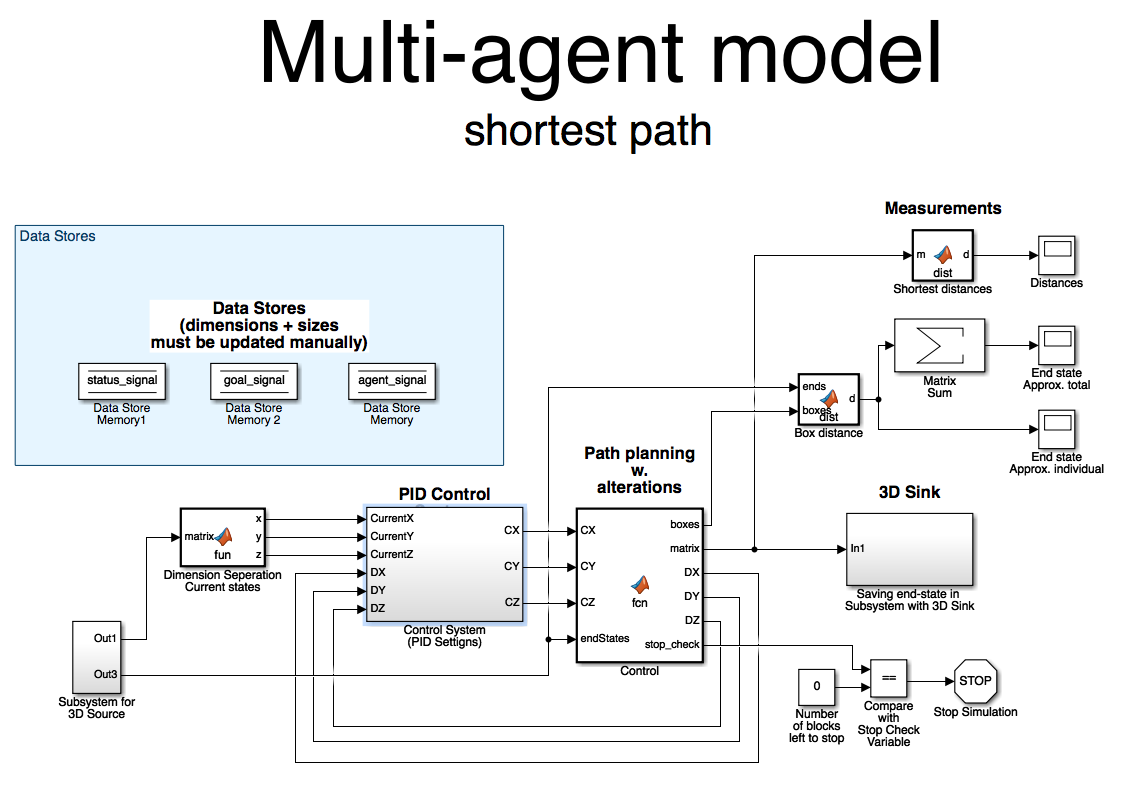
\includegraphics[width=1\columnwidth]{figures/model_overview}
  \caption{\label{fig:model_overview}Overview of finished model in Simulink}
\end{figure}

The following subsections will outline how the different model requirements outlined in Section \ref{sec:physics}, were achieved in a step wise manner.

\subsection{Sources and Sinks}
The simulation is carried out with a start and an endpoint 

\subsection{PID Controller}
As mentioned in Section \ref{sec:simulation_animation}, it is important the control systems cannot alter the position of the quadcopters directly, but instead gives instructions to the quadcopters to change their thrust etc. 

\subsection{Gravity \& Impulse}

\subsection{Control Loop Controller}

\section{Validation}
\label{sec:validation}

\section{Test Metrics}
\label{sec:test_metrics}


